\bfsection{平成31年度 専門科目}

\bfsubsection{問5}
\barquo{
$\C$の部分空間
\[
X = \setmid{1- e^{i\grt} \in \C }{0 \leq \grt < 2\pi} \cup \setmid{-1 + e^{i\grt} \in \C}{0 \leq \grt < 2\pi }
\]
を考える。整数$p,q$に対して、写像$f \colon X \to X$を
\begin{align*}
  f(1- e^{i\grt}) &= -1 + e^{ip\grt} \\
    f(-1 + e^{i\grt}) &= 1 - e^{iq\grt}
\end{align*}
で定め、$X \tm [0,1]$に
\[
(x,0) \sim (f(x),1)
\]
($x \in X$)で生成される同値関係$\sim$を与える。商空間$Y = (X \tm [0,1])/ \sim$の整数係数ホモロジー群を計算せよ。
}
\begin{sol}
\begin{comment}
セル複体を使ってホモロジーを求めよう。空間$Y$を直接書くことは難しいが、次のようなものを想像することはできる。

\begin{center}
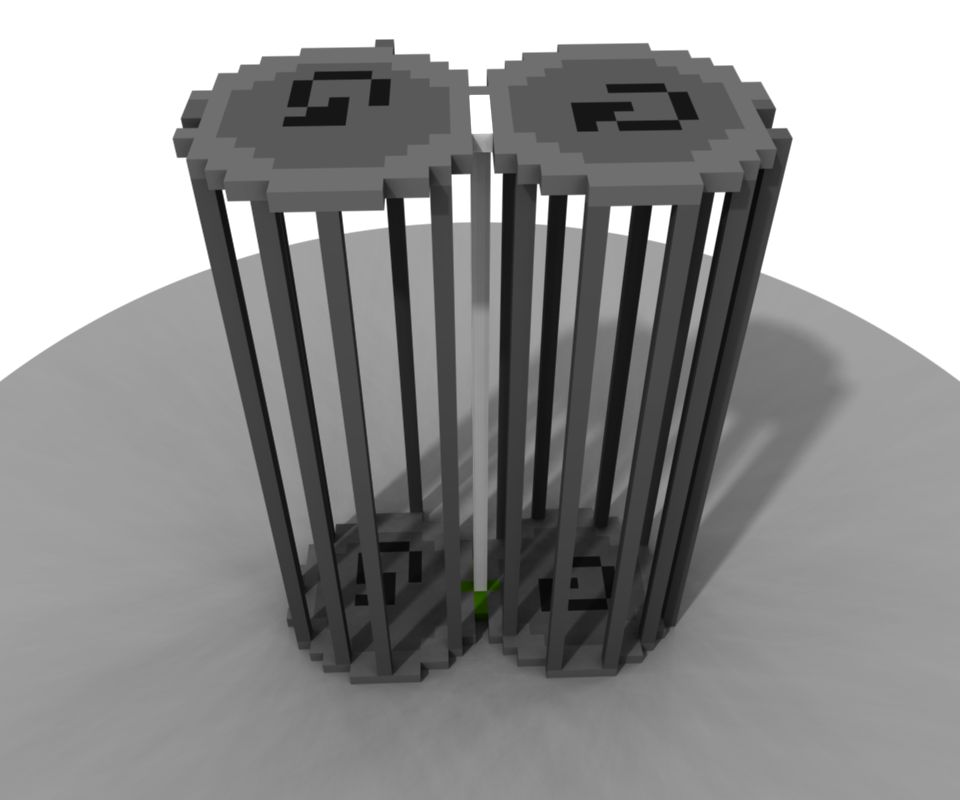
\includegraphics[width=5cm]{strange_object.png}
\end{center}

この対になった円筒は、$X \tm I$を表している。円盤が格子でつながっているかのような図だが、本当は側面もある。垂直方向が$I$成分を表しており、上が$t=0$で下が$t=1$であるものとしよう。また右を実軸のプラス方向、奥を虚軸のプラス方向とする。底の緑の部分は原点を表す。この図形の2-セルは、上下にある4枚の円盤を同一視したものと側面の3つである。向きは図のように定めておく。
\end{comment}
\end{sol}
